%Texlive-full Version 3.141592-1.40.3 (Web2C 7.5.6)
%Kile Version 2.0.83
%File associated : SoFa_Logo.ps , FF.ps

\documentclass[a4paper,10pt]{article}
\usepackage[utf8x]{inputenc}
\usepackage[T1]{fontenc} 

\usepackage{lmodern}
\usepackage[a4paper]{geometry}
%\usepackage[frenchb]{babel}
\usepackage{graphicx}
\usepackage{hyperref}

\usepackage{pstricks}
\usepackage{pst-node}
%\usepackage{wrapfig}
\usepackage{amsmath}
\usepackage{amsfonts}
\usepackage{amssymb}
\usepackage{textcomp}
%\usepackage{mathaccent}
\usepackage{listings}
\lstset{language=C++,basicstyle=\scriptsize \color{green},identifierstyle=\color{orange},keywordstyle=[1]\color{blue},columns=fullflexible,commentstyle=\textit}

\usepackage{color}



\begin{document}
%%%%%%%%%%%%%%%%%%   LOGO  %%%%%%%%%%%%%%%%%%%%%%%%%
\begin{center}
\rput(6,1.5){\href{http://www.sofa-framework.org/}{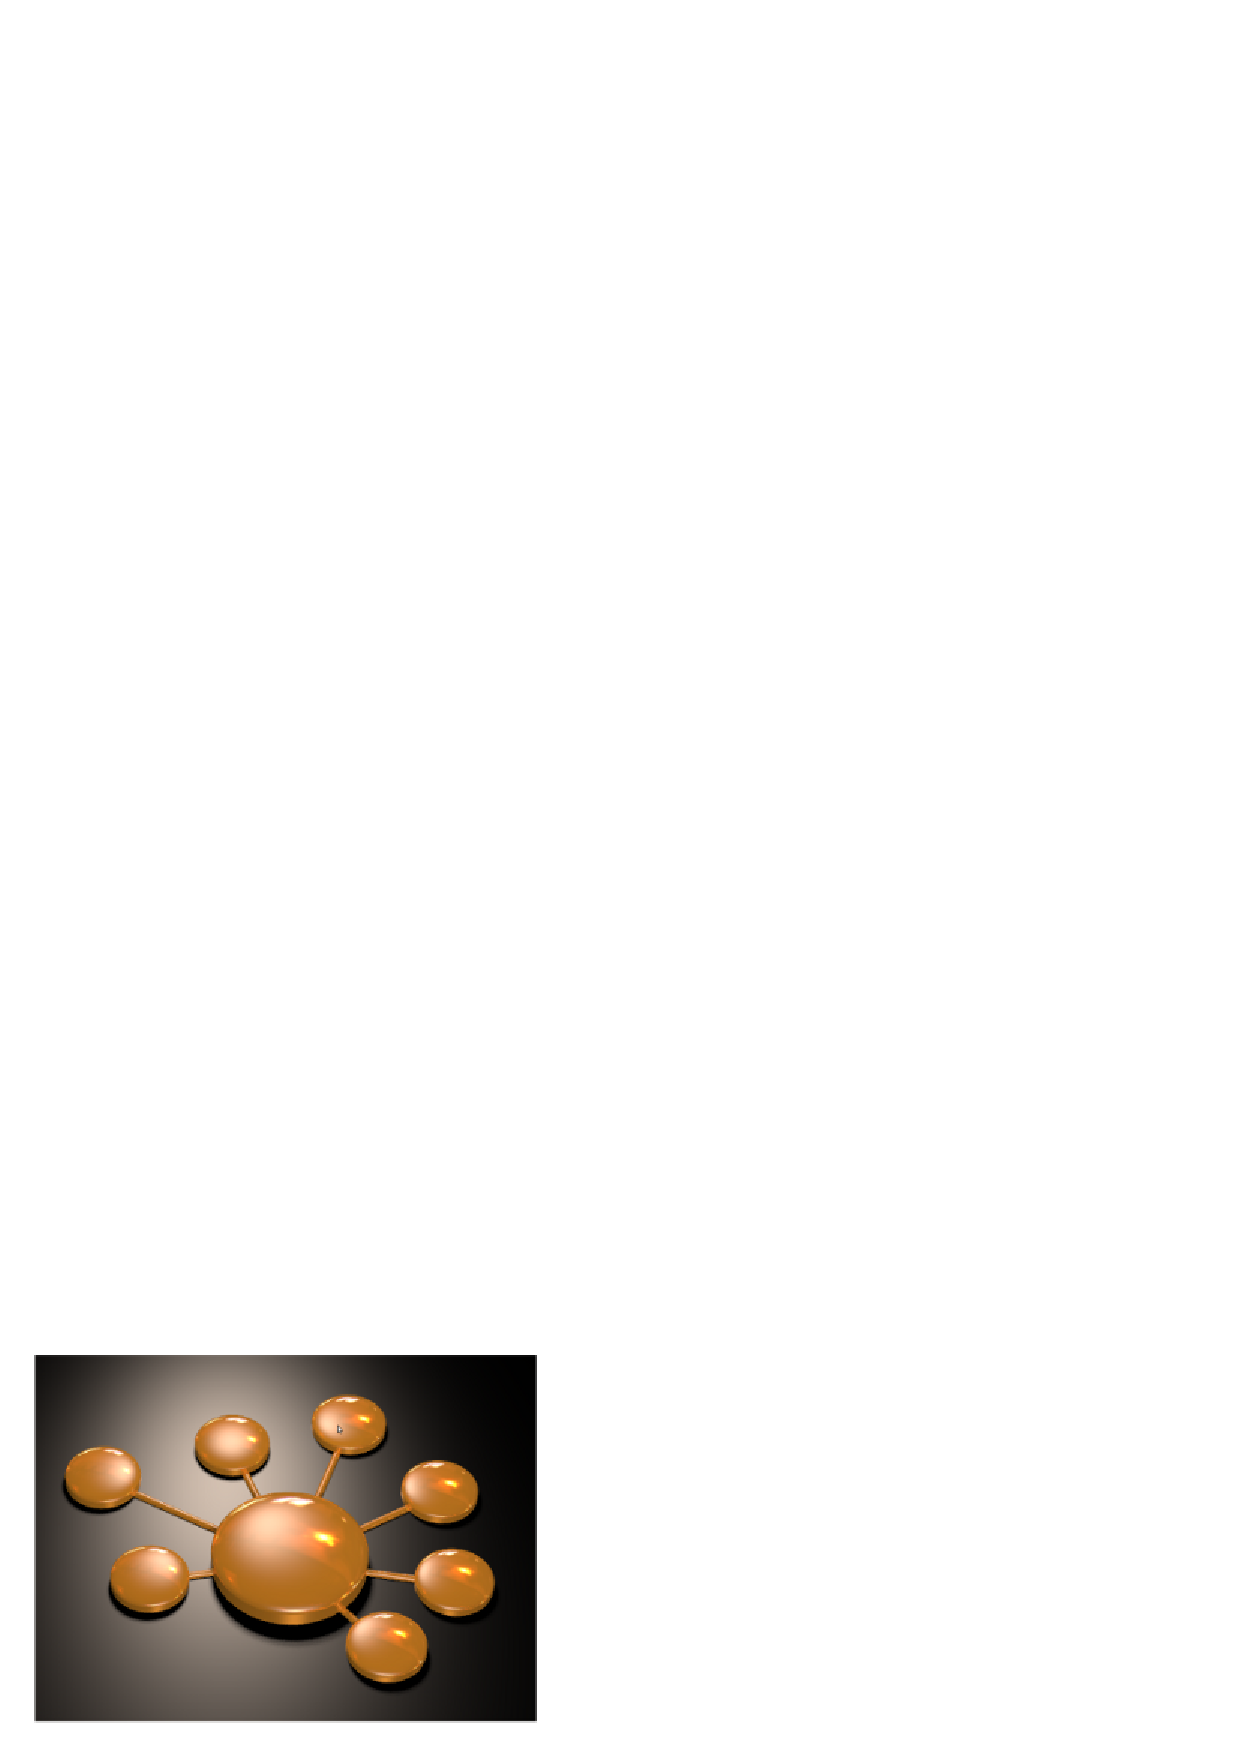
\includegraphics[scale=0.3]{SoFa_Logo}}}
\rput(-4,1.5){\href{http://www.sofa-framework.org/}{
		\begin{tabular}{l}
		\resizebox{4cm}{0.6cm}{SOFA} \\ 
		\resizebox{6cm}{0.3cm}{Simulation Open Framework Architecture}
		\end{tabular}
		}
	    }
\end{center}
%%%%%%%%%%%%%%%%%%   LOGO  %%%%%%%%%%%%%%%%%%%%%%%%%

%%%%%%%%%%%%%%%%%% DOCUMENT TITLE %%%%%%%%%%%%%%%%%%%%%%%%% To be deleted when include in the global document
%\chapter{Mapping} %\section{Rigid Mapping} 
\vspace{1.5cm}
\begin{center}\resizebox{7cm}{0.6cm}{Linear Solver}\end{center}
%%%%%%%%%%%%%%%%%% DOCUMENT TITLE %%%%%%%%%%%%%%%%%%%%%%%%%

%%%%%%%%%%%%%%%%%%%%%%%%%%%%%%%%%%%%%%%%%%%%%%%%%%%%%%%%%%%%%%%%%%%%%%%%%%%%%%%%%%%%%%%%%
%=======================================================================================%
%%%%%%%%%%%%%%%%%%%%%%%%%%%%%%%%%%%%%%%%%%%%%%%%%%%%%%%%%%%%%%%%%%%%%%%%%%%%%%%%%%%%%%%%%
%\section{Linear Solver}% for adding to the global document of SOFA

\section{Linear Solver}
\paragraph{Abstract : }
%%%%%%%%%%%%%%%%%%   LOGO  %%%%%%%%%%%%%%%%%%%%%%%%%
%%%%%%%%%%%%%%%%%%   LOGO  %%%%%%%%%%%%%%%%%%%%%%%%%
In SOFA, all states of a mechanical object is described by its degree of freedom. The relation between theses DOF are informed all in the stiffness matrix. 
\begin{center}
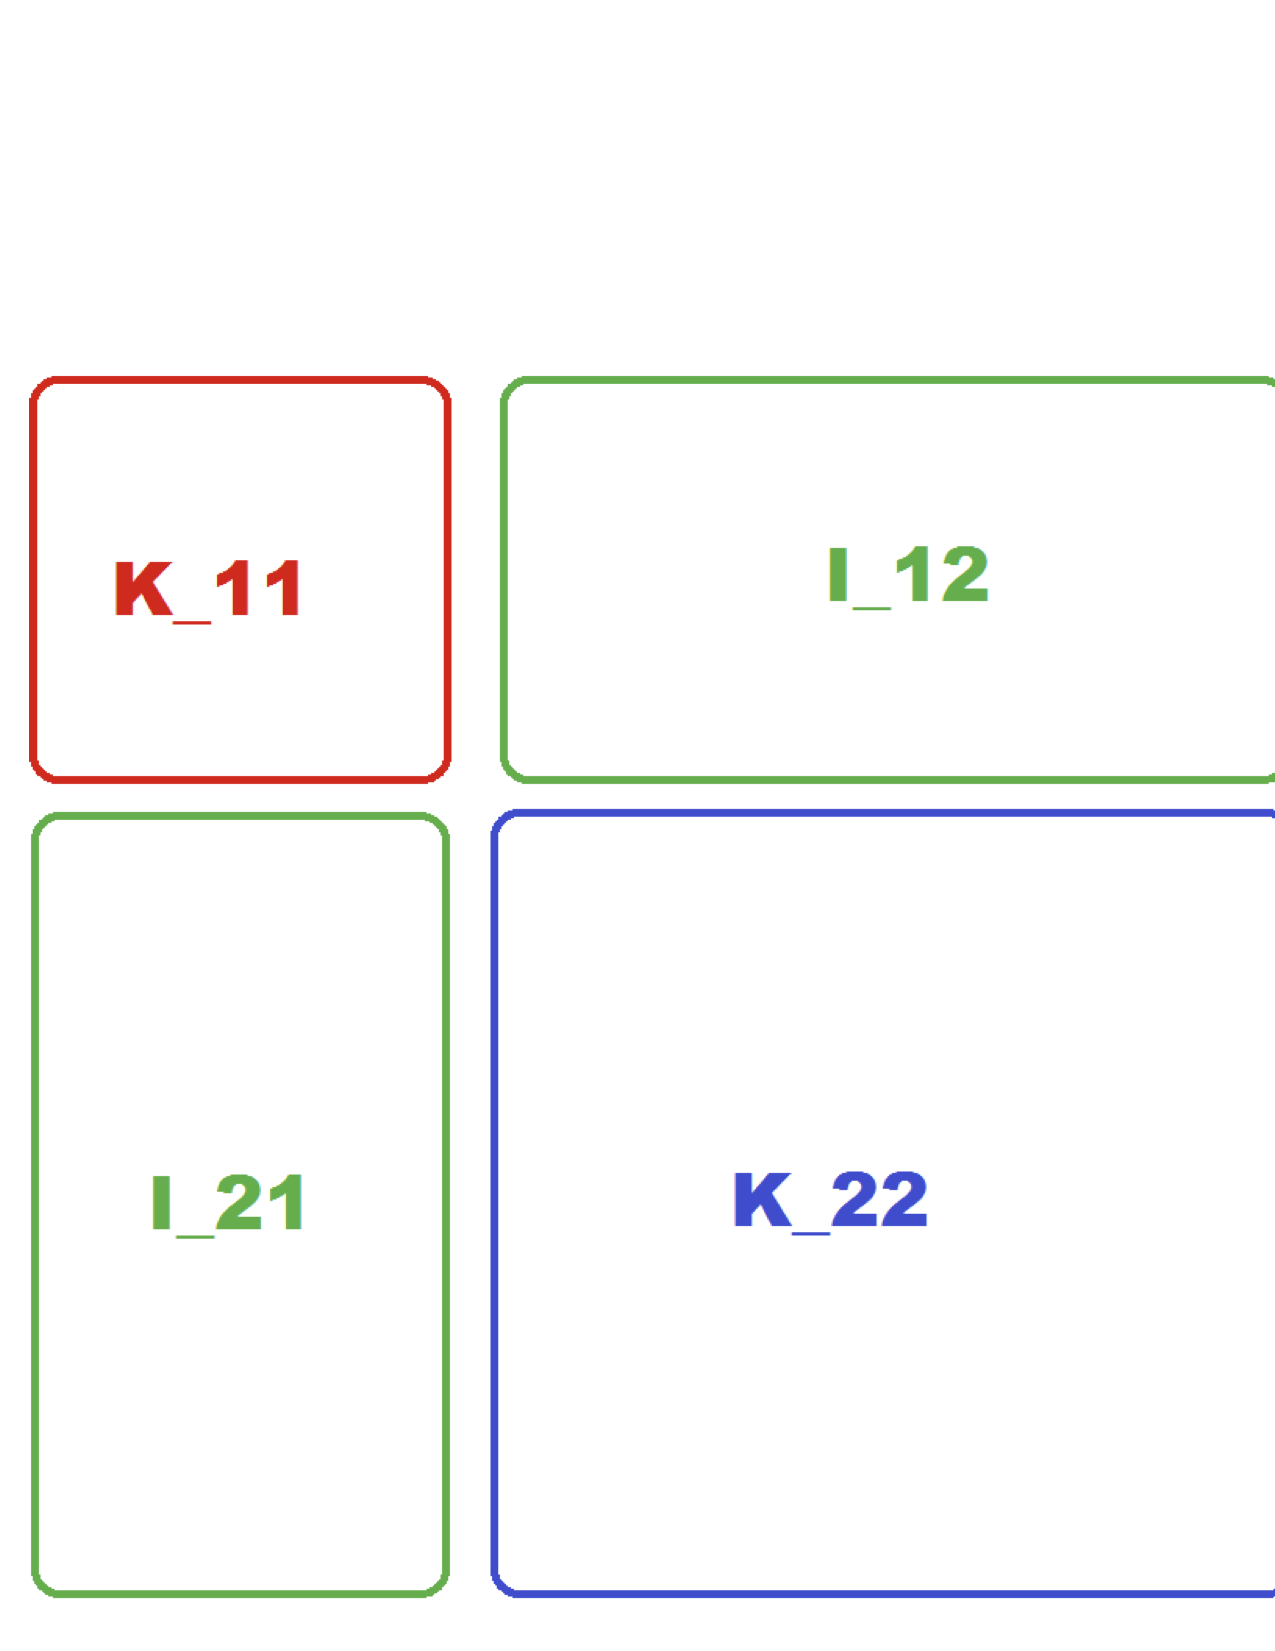
\includegraphics[scale=0.3]{matrix_bloc}
\end{center}
On the case for example when there are two mechanical objects, we can see a global stiffness matrix describing the two mechanical states, composed diagonal blocs and non-diagonal blocs. The diagonal blocs often are filled by ForceField component in SOFA, and the non-diagonal ones are filled by InteractionForceField if existed.
\subsection{Direct Solvers }
The direct solver demande to build explicitly the matrix, and invert this matrix after every step of time in order to solve the mechanical response after a sollicitation.
\subsection{Context in SOFA }
In SOFA, there are a litle more complicated component called mapping, relying geometrical and mechanical propreties by master-slave (DOF-mapped object) relation. All changes of geometry or sollicitation to one object interfere to other and vice versa. If the mapped object have its own mechanical behavior, it must be counted on the mechanical propagation on the mapping.
\subsubsection{self-stiffness propagation }
where the $K_{22}$ is a mapped mechanical state of the $K_{11}$
\begin{center}
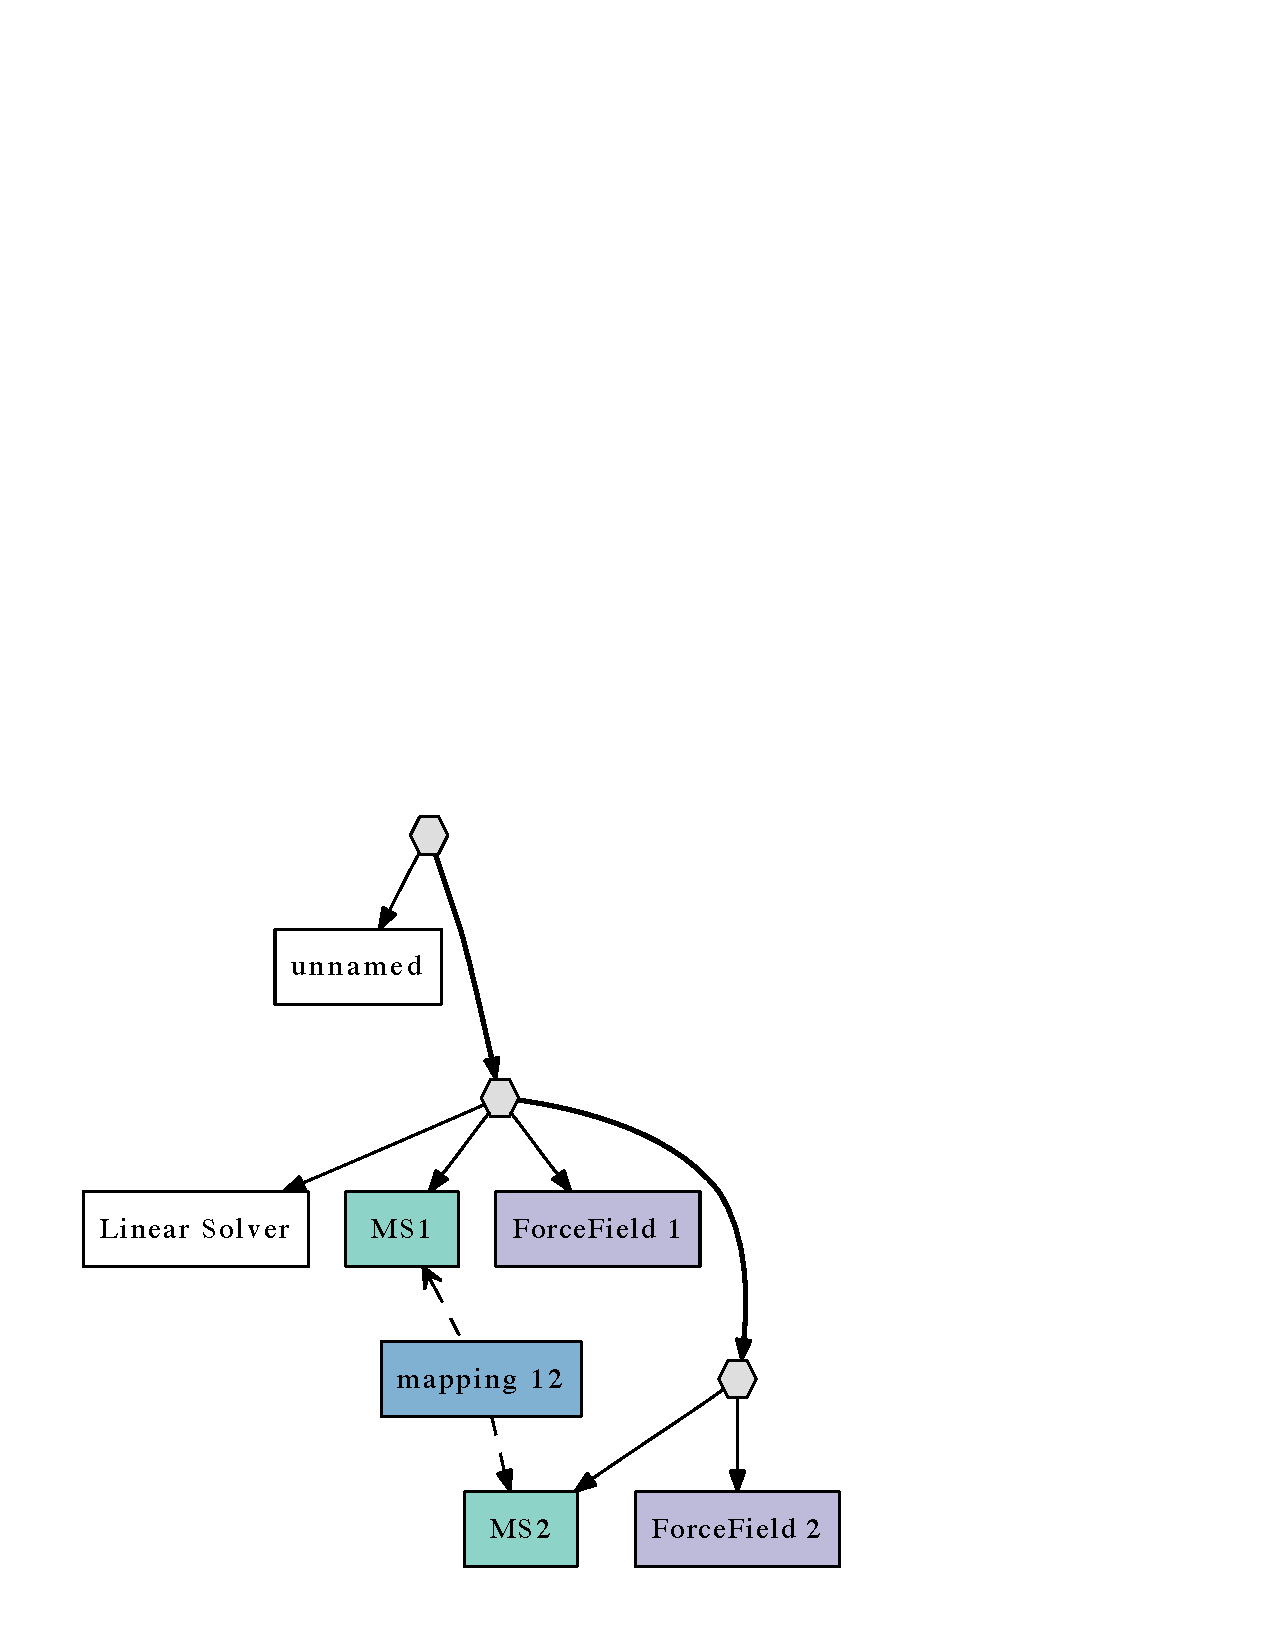
\includegraphics[scale=0.3]{stiffness_propagation}
\end{center}
\[
 K_{11} += J^t * K_{22} * J
\]
\subsubsection{interaction-stiffness propagation }
In the general case, the may have a simulation scene where there are many level of mapped mechanical states (mapped of mapped state ...) and many interaction forcefield interacting beetween them. Therefor the stiffness of interaction forcefield and the mapped mechanical state need to be propagated through the mappings. We can imagine for one propagation, there are two simple cases.
\paragraph{Interaction beweent Real Mechanical Object and Mapped Mechanical Object}
\begin{center}
  \includegraphics[scale=0.3]{interaction_Real_Mapped}
\end{center}
In the case where one of the two mechanical states in interaction is non-mapped, the propagation can be computed directly by the formula :
\[
K_{11} += J^t * K_{33} * J 
\]
\[
I_{12} += J^t * I_{32}
\]
\[
I_{21} += I_{32} * J 
\]
\paragraph{Interaction beweent Mapped Mechanical Object and Mapped Mechanical Object}
\begin{center}
  \includegraphics[scale=0.3]{interaction_Mapped_Mapped}
\end{center}
In the case where the two mechanical states in interaction are mapped, the propagation can be computed by two steps. The first consist to propagate the interaction $I_{34}$ to the interation $I_{14}$ :
\[
K_{11} += J^t * K_{33} * J 
\]
\[
I_{14} += J^t_A * I_{34}
\]
\[
I_{41} += I_{34} * J_A 
\]
The following step can compute as the one of above paragraph, propagating the interation $I_{14}$ to $I_{12}$.
\subsection{Iterative Solvers }
\subsection{Preconditioner }



						      %%%%%%%%%%%%%%%%%%%%%%%%%%  Writer %%%%%%%%%%%%%%%%%%%%%%%%
						      \begin{flushright}
						      Document written by \\
						      \href{mailto:chi-thanh.nguyen@inria.fr}{{\textbf {Chi Thanh NGUYEN}}} \\
						      INRIA Lille
						      \end{flushright}
						      %%%%%%%%%%%%%%%%%%%%%%%%%%  Writer %%%%%%%%%%%%%%%%%%%%%%%%

%\bibliographystyle{siam}
%\bibliography{mybiblio}
\end{document}
